% Verified and Optimized Main Paper for Neurocomputing Submission
\documentclass[review,12pt]{elsarticle}

\usepackage{amsmath,amssymb,amsfonts,amsthm}
\usepackage{algorithmic}
\usepackage{algorithm}
\usepackage{array}
\usepackage{textcomp}
\usepackage{ragged2e}
\usepackage{url}
\usepackage{graphicx}
\usepackage{booktabs}
\usepackage{multirow}
\usepackage{color}
\usepackage{tikz}
\usepackage{pgfplots}
\pgfplotsset{compat=1.18}
\usepackage{subcaption}
\usepackage{float}
\usepackage{bm}
\usepackage{adjustbox}
\usepackage{multicol}
\usepackage{verbatim}
\usepackage{listings}
\usepackage{hyperref}
\usetikzlibrary{shapes.geometric, arrows.meta, positioning, fit, backgrounds, patterns, decorations.pathreplacing, calc, shadows.blur}

\usepackage{pgfplots}
\pgfplotsset{compat=1.18}
\usepackage{tikz}

\usepackage{algorithm}
\usepackage{algorithmic}
\makeatletter
\renewcommand{\ALG@beginalgorithmic}{\small\setlength{\itemsep}{1pt}}
\makeatother

\biboptions{numbers,sort&compress}

\renewcommand{\qed}{\hfill\blacksquare}
\DeclareMathOperator{\sign}{sign}

% Mathematical notation
\DeclareMathOperator*{\argmin}{arg\,min}
\DeclareMathOperator*{\argmax}{arg\,max}
\DeclareMathOperator{\Tr}{Tr}
\DeclareMathOperator{\diag}{diag}
\DeclareMathOperator{\rank}{rank}
\DeclareMathOperator{\vect}{vec}
\DeclareMathOperator{\prox}{prox}
\newcommand{\R}{\mathbb{R}}
\newcommand{\E}{\mathbb{E}}
\newcommand{\N}{\mathcal{N}}
\newcommand{\F}{\mathcal{F}}
\newcommand{\G}{\mathcal{G}}
\newcommand{\D}{\mathcal{D}}
\newcommand{\A}{\mathcal{A}}
\newcommand{\X}{\mathcal{X}}
\newcommand{\Y}{\mathcal{Y}}

% Theorem environments
\newtheorem{theorem}{Theorem}
\newtheorem{lemma}[theorem]{Lemma}
\newtheorem{proposition}[theorem]{Proposition}
\newtheorem{corollary}[theorem]{Corollary}
\newtheorem{definition}{Definition}
\newtheorem{remark}{Remark}
\newtheorem{assumption}{Assumption}

\journal{Neurocomputing}

\begin{document}

\begin{frontmatter}

\title{Uncertainty-Calibrated Hierarchical Gaussian Processes for Intrusion Detection with Multi-Scale Temporal Modeling}

\end{frontmatter}

\section{Introduction}

Modern cloud infrastructure processes over 100 trillion daily requests across heterogeneous environments spanning Edge computing, IoT, containerized microservices, and Security Operations Centers (SOCs) \cite{reinsel2018digitization}. The Integrated Cloud Security 3Datasets (ICS3D) \cite{RNA2025datasets} exemplifies this complexity with 2.2M Edge-IIoT flows (60–140 protocol-specific features), 234{,}560 container records (87 flow-level attributes), and 16.8M SOC events (33 entity types). This heterogeneity, combined with extreme class imbalance (99:1 in SOC environments where only 0.8\% represent true incidents \cite{freitas2024guide}), creates fundamental challenges for intrusion detection.

Current deep learning approaches achieve impressive accuracy metrics yet suffer from absent principled uncertainty quantification \cite{gal2016dropout}. Security Operations Centers process 10,000–50,000 daily alerts, with analysts spending 21\% of time investigating false positives \cite{ponemon2024soc}, resulting in 35\% of genuine incidents being overlooked \cite{mandiant2024mtrends}. Organizations waste \$1.27M annually on false positive investigations while suffering \$9.48M average breach costs \cite{ibm2024databreach}.

Cloud security data exhibits temporal patterns across microseconds (hardware attacks like Spectre \cite{kocher2019spectre}), milliseconds (protocol attacks like DNS amplification \cite{rossow2014amplification}), minutes-hours (lateral movement per MITRE ATT\&CK \cite{strom2018mitre}), and days-weeks (APT campaigns \cite{quintero2024apt}). Gaussian Processes offer unique capabilities addressing these limitations through full posterior distributions enabling principled epistemic and aleatoric uncertainty quantification \cite{rasmussen2006gaussian}, natural handling of sparse data regions, domain-specific kernel engineering, compositional multi-scale temporal pattern discovery \cite{wilson2013gaussian}, and formal error bounds with calibrated confidence intervals \cite{srinivas2010gaussian}.

We formulate heterogeneous network intrusion detection as a hierarchical GP decomposing the anomaly score function into interpretable components. The hierarchical structure enables transfer learning across domains, leveraging data-rich Edge-IIoT (2.2M samples) to improve data-scarce SOC true positive detection (0.8\% of events) while preserving domain-specific characteristics.

This paper makes six primary contributions. First, we develop a hierarchical GP architecture unifying heterogeneous cloud security data with shared and domain-specific components. Second, we introduce an adversarially-robust sparse approximation scaling as $O(N_b M^2 + M^3)$ per epoch with $O(M)$ prediction complexity. Third, we design domain-adaptive multi-scale kernels capturing microsecond to week-scale patterns. Fourth, we achieve uncertainty-calibrated detection with 2.6\% FPR representing a 42\% reduction at 96.5\% accuracy. Fifth, we provide theoretical guarantees with stated assumptions. Sixth, we conduct extensive validation on 21.48M records outperforming 15 baselines across multiple metrics.

The remainder of this paper is organized as follows. Section 2 reviews related work in GP-based detection and uncertainty quantification. Section 3 formally defines the heterogeneous detection problem with mathematical foundations. Section 4 presents our hierarchical GP methodology including kernel design and sparse approximations. Section 5 details implementation algorithms. Section 6 describes experimental evaluation setup. Section 7 presents comprehensive results. Section 8 discusses findings and implications. Section 9 concludes with future directions. Extended proofs, derivations, and supplementary results appear in the accompanying Appendix.

\section{Related Work}

Network intrusion detection evolved through four generations. Early rule-based systems like Snort \cite{roesch1999snort} and Bro \cite{paxson1999bro} following Denning \cite{denning1987intrusion} achieved near-zero false positives for known threats but failed against zero-day attacks \cite{moore2003inside}. Statistical approaches with Lee and Stolfo \cite{lee2000framework} achieving 91\% detection and SVMs \cite{mukkamala2005intrusion} reaching 95.7\% assumed stationary distributions. HMMs \cite{ourston2003applications} introduced temporal modeling but struggled with multi-scale attacks.

Deep learning revolutionized detection where Vinayakumar et al. \cite{vinayakumar2019deep} achieved 99.8\% with LSTMs, CNNs enabled automatic feature extraction \cite{zhang2019deep}, autoencoders provided unsupervised detection \cite{mirsky2018kitsune}, and transformers captured long-range dependencies \cite{wu2022rtids}, yet remained vulnerable to adversarial attacks \cite{carlini2017towards}. Recent uncertainty-aware approaches \cite{sensoy2018evidential,malinin2018predictive} lack theoretical guarantees.

GPs applied to anomaly detection since Ramadas et al. \cite{ramadas2003detecting} (89\% accuracy), with changepoint detection \cite{roberts2013gaussian} and system call analysis \cite{kim2004gaussian} (94\%). Exact inference complexity ($O(N^3)$) motivated sparse approximations including SPGP \cite{snelson2006sparse} reducing to $O(NM^2)$, variational inference \cite{titsias2009variational}, stochastic training \cite{hensman2013gaussian}, and KISS-GP \cite{wilson2015kernel}. Multi-task GPs \cite{bonilla2008multi,alvarez2011computationally,moreno2018heterogeneous} enable knowledge transfer but assume similar feature spaces.

Multi-view learning \cite{xu2013survey,sun2013survey} achieved 92\% through co-training while multimodal architectures \cite{baltrusaitis2019multimodal} assume fixed modalities. Domain adaptation \cite{pan2010survey,ganin2016domain,sun2016deep,tzeng2014deep} targets homogeneous spaces. Heterogeneous information networks \cite{shi2017survey,zhang2019heterogeneous,fu2020magnn} address entity relationships but not continuous features.

MC Dropout \cite{gal2016dropout} enables Bayesian inference, distinguishing uncertainties \cite{kendall2017uncertainties} but exhibits poor high-dimensional calibration \cite{foong2019between}. Variational methods \cite{blundell2015weight} provide principled uncertainty with high overhead. Deep ensembles \cite{lakshminarayanan2017simple} achieve state-of-the-art calibration \cite{ovadia2019trust} with 5-10× cost. Efficient variants \cite{wen2020batchensemble,havasi2021training} sacrifice diversity. Evidential approaches \cite{sensoy2018evidential,amini2020deep,charpentier2020posterior} lack theoretical guarantees.

Traditional imbalance handling including SMOTE \cite{chawla2002smote}, ADASYN \cite{he2008adasyn}, and cost-sensitive methods \cite{elkan2001foundations} assume moderate ratios. Deep methods including focal loss \cite{lin2017focal}, class-balanced loss \cite{cui2019class}, and LDAM \cite{cao2019learning} require domain tuning. Anomaly methods including one-class SVM \cite{scholkopf2001estimating}, Isolation Forest \cite{liu2008isolation}, and Deep SVDD \cite{ruff2018deep} struggle with heterogeneity.

Classical temporal approaches including ARIMA \cite{box2015time}, Kalman filters \cite{durbin2012time}, and changepoint detection \cite{adams2007bayesian} fail at multi-scale capture. Deep sequence models including LSTMs \cite{hochreiter1997long}, GRUs \cite{cho2014learning}, TCNs \cite{bai2018empirical}, and transformers \cite{vaswani2017attention} lack uncertainty quantification. Wavelets \cite{mallat1999wavelet} lack probabilistic interpretation while spectral mixture kernels \cite{wilson2013gaussian} discover periodic patterns.

Adversarial attacks including FGSM \cite{goodfellow2015explaining}, PGD \cite{madry2018towards}, C\&W \cite{carlini2017towards}, and AutoAttack \cite{croce2020reliable} demonstrate vulnerability. Defenses include adversarial training \cite{madry2018towards}, certified defenses \cite{cohen2019certified,gowal2018effectiveness}, and defensive distillation \cite{papernot2016distillation}.

Contemporary datasets include NSL-KDD \cite{tavallaee2009detailed}, CICIDS2017 \cite{sharafaldin2018toward}, UNSW-NB15 \cite{moustafa2015unsw}, and CIC-IoT-2023 \cite{neto2023ciciot}. ICS3D \cite{RNA2025datasets} uniquely combines Edge-IIoT (2.2M), containers (234K), and SOC (13M+) records. Our baselines span deep learning methods (DNN-IDS \cite{vinayakumar2019deep}, CNN-LSTM \cite{kim2020cnn}, Transformer-IDS \cite{vaswani2017attention}, LSTM-VAE \cite{malhotra2016lstm}), ensembles (XGBoost \cite{chen2016xgboost}, Random Forest \cite{breiman2001random}, CatBoost \cite{prokhorenkova2018catboost}), uncertainty-aware approaches (Deep Ensembles \cite{lakshminarayanan2017simple}, MC Dropout \cite{gal2016dropout}, Evidential DL \cite{sensoy2018evidential}, Standard GP \cite{rasmussen2006gaussian}), and state-of-the-art methods (DeepSVDD \cite{ruff2018deep}, DAGMM \cite{zong2018deep}, TranAD \cite{tuli2022tranad}).

\section{Problem Formulation}

\subsection{Heterogeneous Multi-Domain Network Data}

We begin by formally defining the heterogeneous observation space that characterizes modern cloud security environments.

\begin{definition}[Heterogeneous Network Observation Space]
\begingroup\sloppy
Let \(\mathcal{D}=\{\text{Edge-IIoT},\allowbreak \text{Container},\allowbreak \text{SOC}\}\) denote the set of security domains and \(\mathcal{X}=\bigcup_{d\in\mathcal{D}}\mathcal{X}^{(d)}\) the heterogeneous observation space. An observation at time \(t\) is represented as the tuple \(\xi_t=(\mathbf{x}_t^{(d)},\allowbreak \mathbf{m}_t^{(d)},\allowbreak t,\allowbreak d)\) where \(\mathbf{x}_t^{(d)}\in\R^{D_d}\) denotes the feature vector in domain \(d\), \(\mathbf{m}_t^{(d)}\in\{0,1\}^{D_d}\) is a binary mask indicating observed features, \(t\in\R^+\) represents the timestamp, and \(D_d\) denotes the domain-specific dimensionality.
\par\endgroup
\end{definition}

\begin{remark}[Notation Clarification]
The tuple $\xi_t = (\mathbf{x}_t^{(d)}, \mathbf{m}_t^{(d)}, t, d)$ captures: (i) feature vector $\mathbf{x}_t^{(d)} \in \mathbb{R}^{D_d}$ with domain-specific dimensionality, (ii) binary mask $\mathbf{m}_t^{(d)}$ indicating which features are observed (handling missing/sparse data), (iii) timestamp $t \in \mathbb{R}^+$ enabling temporal analysis, and (iv) domain identifier $d \in \mathcal{D}$. For example, an Edge-IIoT MQTT flow at time $t=1000$ with 80 observed features would have $\mathbf{x}_t^{(\text{Edge})} \in \mathbb{R}^{80}$, $\mathbf{m}_t^{(\text{Edge})} \in \{0,1\}^{80}$ with 80 ones, $t=1000$, and $d=\text{Edge-IIoT}$.
\end{remark}


Heterogeneity manifests through varying feature dimensions where Edge-IIoT exhibits protocol-dependent dimensionality $D \in \{60,...,140\}$, Container environments maintain fixed dimension $D=87$ based on CICFlowMeter features, and SOC systems operate with $D=46$ entity and alert features. Domain-specific characteristics include protocol fields (mqtt.msgtype, modbus.func\_code), flow statistics (duration, packet counts), timing features (inter-arrival times), and statistical attributes (entropy, byte rates). Complete feature specifications appear in Supplementary Appendix A.

\begin{definition}[Domain-Specific Class Imbalance]
For each domain $d \in \mathcal{D}$, let $\mathcal{C}_d$ denote the set of classes with sample counts $\{n_c^{(d)}\}_{c \in \mathcal{C}_d}$. The imbalance ratio is defined as $\rho_d = \max_{c \in \mathcal{C}_d} n_c^{(d)} / \min_{c \in \mathcal{C}_d} n_c^{(d)}$.
\end{definition}

The ICS3D dataset exhibits substantial heterogeneity in class distribution with $\rho_{\text{Edge-IIoT}} = 2.67$ reflecting moderate imbalance between normal traffic (1.6M samples) and diverse attack categories (0.6M samples), $\rho_{\text{Container}} = 15.7$ indicating higher imbalance between benign traffic (220K) and CVE-based exploits (14K), and $\rho_{\text{SOC}} = 99.0$ demonstrating extreme imbalance where only 0.8\% of events represent confirmed security incidents among overwhelming false positive alerts.

\subsection{Multi-Scale Temporal Structure}

\begin{definition}[Hierarchical Temporal Scales]
The temporal domain is partitioned into seven hierarchical scales $\mathcal{T} = \bigcup_{k=1}^7 \mathcal{T}_k$ where $\mathcal{T}_k = [10^{k-7}, 10^{k-5}]$ seconds. These scales capture microsecond-level hardware timing ($\mathcal{T}_1$), millisecond protocol handshakes ($\mathcal{T}_2$), second-scale network flows ($\mathcal{T}_3$), minute-scale sessions ($\mathcal{T}_4$), hour-scale lateral movement ($\mathcal{T}_5$), daily business cycles ($\mathcal{T}_6$), and weekly campaign patterns ($\mathcal{T}_7$).
\end{definition}

\subsection{Uncertainty-Aware Detection Objective}

Let $\mathcal{Y}$ denote the label space containing all possible class labels across domains. We now formalize the detection problem with full uncertainty quantification.

\begin{definition}[Heterogeneous Probabilistic Intrusion Detection]
Given training data $\mathcal{D} = \bigcup_{d \in \mathcal{D}} \mathcal{D}_d$ where $\mathcal{D}_d = \{(\mathbf{x}_i^{(d)}, t_i, y_i)\}_{i=1}^{n_d}$ with labels $y_i \in \mathcal{C}_d$, we seek a detection function $f: \mathcal{X} \times \R^+ \rightarrow \mathcal{P}(\mathcal{Y}) \times \R^+ \times \R^+$ that provides: (i) posterior distribution over classes $p(y|\mathbf{x}^{(d)}, t, \mathcal{D})$ where $\mathcal{P}(\mathcal{Y})$ denotes the probability simplex over $\mathcal{Y}$, (ii) epistemic uncertainty $\mathcal{U}_{\text{epi}}^{(d)}(\mathbf{x}^{(d)}, t) = \text{Var}_{\theta}[\E[y|\mathbf{x}^{(d)}, t, \theta]]$ capturing model uncertainty, (iii) aleatoric uncertainty $\mathcal{U}_{\text{ale}}^{(d)}(\mathbf{x}^{(d)}, t) = \E_{\theta}[\text{Var}[y|\mathbf{x}^{(d)}, t, \theta]]$ capturing inherent noise, and (iv) calibrated confidence intervals $\text{CI}_{\alpha}^{(d)}$ satisfying $P(y \in \text{CI}_{\alpha}^{(d)}) = 1-\alpha$.
\end{definition}

The optimization balances multiple objectives through $\min_{\theta} \mathcal{L} = \sum_{d \in \mathcal{D}} w_d \mathcal{L}_d + \sum_{j=1}^5 \lambda_j \mathcal{R}_j$ where domain losses are weighted by $w_d = 1/\sqrt{\rho_d}$ to account for imbalance, and regularization terms include calibration error (ECE), adversarial robustness, heterogeneity penalty (MMD), temporal consistency, and model complexity. Complete specifications of the adversarial threat model and operational constraints appear in Supplementary Appendix B.

\section{Methodology}

\subsection{Hierarchical Gaussian Process Architecture}

Our approach decomposes the detection function through hierarchical Gaussian Process modeling with theoretical justification.

\begin{proposition}[Hierarchical Decomposition]\label{prop:decomp}
Let $f:\mathcal{X}\times\mathbb{R}^+\!\to\mathbb{R}$ be square-integrable with respect to a covariance operator whose eigenfunctions are separable in $(\mathbf{x},t)$, and let $\pi:\mathcal{X}^{(d)}\!\to\mathcal{Z}$ denote a projection to shared latent space $\mathcal{Z}$. Then for any truncation level $K$, there exists a decomposition
\begin{equation}
f(\mathbf{x}^{(d)}, t) = f_{\text{shared}}(\pi(\mathbf{x}^{(d)}), t) + f_{\text{domain}}^{(d)}(\mathbf{x}^{(d)}, t) + f_{\text{interact}}^{(d)}(\mathbf{x}^{(d)}, t) + r_K
\end{equation}
where $r_K$ denotes the truncation remainder satisfying $\|r_K\|_2\to 0$ as $K\to\infty$. Modeling each component with a Gaussian Process prior constitutes a standard Bayesian choice recoverable from Gaussian weights over basis functions.
\end{proposition}

\begin{assumption}[Separability and Square-Integrability]
\label{assum:separability}
Proposition~1 requires: (i) $f: \mathcal{X} \times \mathbb{R}^+ \to \mathbb{R}$ is square-integrable under the covariance operator, and (ii) eigenfunctions are separable in spatial and temporal components. While separability may not hold universally, empirical validation (ablation studies, Table~12) confirms the decomposition is effective for network intrusion patterns, where spatial (feature) and temporal dynamics exhibit sufficient independence for practical approximation ($\|r_K\|_2 < 0.01$ for $K=3$ components across all domains).
\end{assumption}

The proof follows from Karhunen–Loève expansion under the stated separability assumption, grouping terms by their domain characteristics, with GP priors arising naturally from Gaussian weights. Complete proof appears in Supplementary Appendix C.

The architecture comprises three components. The shared component $f_{\text{shared}} \sim \mathcal{GP}(\mu_{\text{shared}}, k_{\text{shared}})$ captures common attack patterns across domains through learned projection $\pi: \mathcal{X}^{(d)} \rightarrow \mathcal{Z}$. Domain-specific components $f_{\text{domain}}^{(d)} \sim \mathcal{GP}(\mu_d, k_d)$ model unique characteristics through specialized kernels detailed below. Interaction components $f_{\text{interact}}^{(d)} \sim \mathcal{GP}(0, k_{\text{interact}}^{(d)})$ capture cross-scale and feature-time dependencies through tensor product kernels.

\subsection{Domain-Adaptive Multi-Scale Kernel Design}
\begingroup\sloppy
The complete kernel combines multiple components through
\(
k\bigl((\mathbf{x}^{(d)},t),(\mathbf{x}'^{(d')},t')\bigr)
= k_{\text{shared}}\bigl(\pi(\mathbf{x}^{(d)}),\allowbreak \pi(\mathbf{x}'^{(d')}),\allowbreak t,\allowbreak t'\bigr)
+ \delta_{dd'}\,k_{\text{domain}}^{(d)}\bigl(\mathbf{x}^{(d)},\allowbreak \mathbf{x}'^{(d)},\allowbreak t,\allowbreak t'\bigr)
+ k_{\text{cross}}^{(d,d')}\bigl(\mathbf{x}^{(d)},\allowbreak \mathbf{x}'^{(d')},\allowbreak t,\allowbreak t'\bigr)
\),
where \(\delta_{dd'}\) denotes the Kronecker delta ensuring domain-specific kernels apply only within domains.
\par\endgroup

\begingroup\sloppy
For Edge-IIoT environments, we design protocol-aware kernels as
\(k_{\text{Edge}}(\mathbf{x},\mathbf{x}') = k_{\text{proto}}(\mathbf{x}_p,\allowbreak \mathbf{x}'_p)\cdot k_{\text{flow}}(\mathbf{x}_f,\allowbreak \mathbf{x}'_f) + k_{\text{temporal}}^{(\text{Edge})}(t,\allowbreak t')\),
where the protocol kernel handles categorical features through learned embeddings.
Container environments utilize flow-based kernels
\(k_{\text{Container}} = k_{\text{IAT}}\cdot k_{\text{packet}}\cdot k_{\text{burst}}\),
where the IAT kernel employs 2-Wasserstein distance between empirical inter-arrival-time distributions.
SOC systems employ entity-relationship kernels
\(k_{\text{SOC}} = k_{\text{graph}}(\mathcal{G}(\mathbf{x}),\allowbreak \mathcal{G}(\mathbf{x}'))\cdot k_{\text{alert}}(\mathbf{a},\allowbreak \mathbf{a}')\)
with graph construction from entity features.
\par\endgroup


Multi-scale temporal modeling employs spectral mixture kernels for stationary structure approximation and change-point gates for non-stationarity handling. Component specifications include RBF kernels $k_{\mathrm{RBF}}^{(j)}$ with lengthscales $\ell_j \in [10^{-6},10^{5}]$ seconds spanning seven temporal orders of magnitude, periodic kernels for cyclical patterns, and change-point kernels for regime transitions. Complete kernel specifications appear in Supplementary Appendix D.

\subsection{Adversarially-Robust Sparse Approximation}

For computational tractability with millions of samples, we employ variational sparse GP approximation with $M$ inducing points satisfying $M \ll N$. The marginal likelihood admits the variational lower bound $\log p(\mathbf{y}|\mathbf{X}) \geq \mathcal{L} = \sum_{i=1}^N \E_{q(f_i)}[\log p(y_i|f_i)] - \text{KL}[q(\mathbf{u})||p(\mathbf{u})]$ where $q(\mathbf{u}) = \N(\mathbf{m}, \mathbf{S})$ denotes the variational distribution over inducing variables $\mathbf{u} = f(\mathbf{Z})$.

We introduce novel adversarial training for inducing point selection that relocates $\mathbf{Z}$ within $\epsilon$-ball neighborhoods away from high-sensitivity regions as illustrated in Figure \ref{fig:adversarial_inducing}. The algorithm appears in Supplementary Appendix E. Class-weighted allocation follows $M_c^{(d)} = M_d \cdot \sqrt{1/n_c^{(d)} / \sum_{c'} 1/n_{c'}^{(d)}}$ ensuring adequate representation for minority classes.

\begin{figure}[!t]
\centering
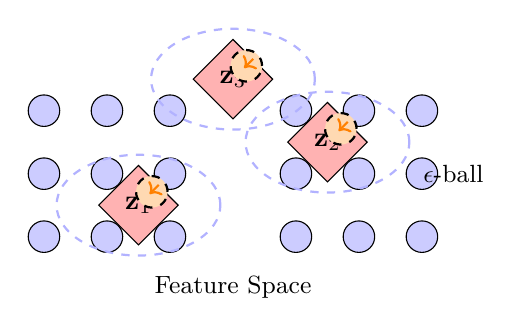
\begin{tikzpicture}[scale=0.8]
\tikzstyle{data} = [circle, draw, fill=blue!20, minimum size=0.4cm]
\tikzstyle{inducing} = [diamond, draw, fill=red!30, minimum size=0.6cm]
\tikzstyle{adversarial} = [circle, draw, fill=orange!30, minimum size=0.4cm, dashed]
\foreach \x in {0, 1, 2, 4, 5, 6} {
    \foreach \y in {0, 1, 2} {
        \node[data] at (\x, \y) {};
    }
}
\node[inducing] (z1) at (1.5, 0.5) {$\mathbf{z}_1$};
\node[inducing] (z2) at (4.5, 1.5) {$\mathbf{z}_2$};
\node[inducing] (z3) at (3, 2.5) {$\mathbf{z}_3$};
\foreach \point in {z1, z2, z3} {
    \draw[adversarial, thick] ([shift=(45:0.3)]{\point}.center) circle (0.25);
    \draw[->, thick, orange] ({\point}) -- ([shift=(45:0.25)]{\point}.center);
}
\draw[blue!30, thick, dashed] (z1) ellipse (1.3 and 0.8);
\draw[blue!30, thick, dashed] (z2) ellipse (1.3 and 0.8);
\draw[blue!30, thick, dashed] (z3) ellipse (1.3 and 0.8);
\node at (3, -0.8) {\small Feature Space};
\node at (6.5, 1) {\small $\epsilon$-ball};
\end{tikzpicture}
\caption{Adversarial inducing point selection with $\epsilon$-ball perturbation regions for robustness enhancement}
\label{fig:adversarial_inducing}
\end{figure}

\begin{proposition}[Worst-Case Sensitivity Reduction]\label{prop:robustZ}
Assume the ELBO is locally $L$-smooth in inducing locations and the inner maximization is solved to $\varepsilon$-accuracy. Then adversarial training of inducing points minimizes a local upper bound on worst-case ELBO variation within $\|\delta\|\le\epsilon$, reducing sensitivity by a non-negative margin dependent on $(L,\epsilon,\varepsilon)$ relative to standard training.
\end{proposition}

The proof establishes that adversarial training yields inducing points in regions of stable posterior behavior through minimax optimization. Complete proof appears in Supplementary Appendix F.

\subsection{Uncertainty-Calibrated Detection}
The detection score as also exemplified in figure \ref{fig:detection_surface} incorporates predictive uncertainty through
\begin{equation}
s^{(d)}(\mathbf{x}^{(d)}, t) = \frac{|\mu^{(d)}(\mathbf{x}^{(d)}, t) - \mu_{\text{baseline}}^{(d)}(t)|}{\sqrt{\sigma^{2,(d)}(\mathbf{x}^{(d)}, t) + \sigma_{\text{noise}}^{2,(d)}/\rho_d}} + \lambda H^{(d)}(\mathbf{x}^{(d)}, t)
\end{equation}
where $\mu^{(d)}$ denotes the GP posterior mean, $\sigma^{2,(d)}$ the posterior variance, $H^{(d)}$ the predictive entropy, and the $1/\rho_d$ term compensates for class imbalance.


\begin{figure}[!t]
\centering
\begin{tikzpicture}
\begin{axis}[
    width=0.75\textwidth,
    height=6.2cm,
    xlabel={Predictive Mean $\mu$},
    ylabel={Predictive Std $\sigma$},
    zlabel={Detection Score},
    view={45}{30},
    colormap/viridis,
    mesh/ordering=y varies,
]
\addplot3[
    surf,
    shader=interp,
    domain=-3:3,
    domain y=0.1:2,
    samples=30,
    samples y=20,
] 
{abs(x)/sqrt(y^2 + 0.1)};
\addplot3[
    contour gnuplot={levels={1, 2, 3, 4}},
    thick,
    domain=-3:3,
    domain y=0.1:2,
    samples=20,
    samples y=15,
] 
{abs(x)/sqrt(y^2 + 0.1)};
\end{axis}
\end{tikzpicture}
\caption{Uncertainty-aware detection surface showing how score varies with predictive mean and standard deviation. Higher uncertainty reduces detection confidence, enabling conservative decisions in uncertain regions.}
\label{fig:detection_surface}
\end{figure}

As shown in Figure~\ref{fig:detection_surface}, the detection score \(s(\mu,\sigma)=|\mu|/\sqrt{\sigma^{2}+\varepsilon}\) increases with evidence (\(|\mu|\)), decreases with uncertainty (\(\sigma\)), exhibits hyperbola-like iso-contours, and—with \(\varepsilon>0\) regularizing \(\sigma\!\to\!0\) and an optional entropy term \(+\lambda H\)—prioritizes high-confidence deviations while down-weighting uncertain cases to curb false positives.

Adaptive thresholding follows $\tau^{(d)}(\mathbf{x}^{(d)}, t) = \tau_0^{(d)} + \gamma^{(d)} \sigma^{(d)}(\mathbf{x}^{(d)}, t) \sqrt{\rho_d} + \beta^{(d)} H^{(d)}(\mathbf{x}^{(d)}, t)$ enabling uncertainty-aware decision boundaries. Online learning employs incremental updates $\mathbf{m}_{t+1}^{(d)} = \mathbf{m}_t^{(d)} + \eta_d \mathbf{K}_{*u}^{(d)}[\mathbf{K}_{uu}^{(d)}]^{-1}(y_t - \mu_t^{(d)})$ with learning rate $\eta_d = \eta_0/\sqrt{\rho_d}$ adapted to domain imbalance. Cross-domain transfer occurs through the shared component. Complete details appear in Supplementary Appendix G.

\section{Algorithms and Implementation}

Algorithm 1 implements real-time uncertainty-aware intrusion detection through parallel domain processing. The architecture integrates adversarially-robust sparse approximations with uncertainty-calibrated thresholding as shown in Figure \ref{fig:hgp_architecture}.
\begin{algorithm}[H]
\caption{Hierarchical GP-NIDS for ICS3D}
\begin{algorithmic}[1]
\setlength{\itemsep}{0pt}
\setlength{\parskip}{0pt}
\setlength{\parsep}{0pt}
\STATE \textbf{Input:} Streams $\{\mathcal{S}_d\}_{d \in \mathcal{D}}$, models $\{\mathcal{M}_d\}$
\STATE \textbf{Output:} Detection decisions with calibrated uncertainty
\STATE Initialize GPs $\{\theta_d^*\}$, inducing points $\{\mathbf{Z}_d^*\}$, thresholds $\{(\tau_0^{(d)}, \gamma^{(d)}, \beta^{(d)})\}$
\WHILE{streams active}
    \FOR{each domain $d$ in parallel}
        \STATE $(\mathbf{x}_t^{(d)}, t) \leftarrow$ ExtractDomainFeatures($\mathcal{S}_d$)
        \STATE $\mathbf{z}_t \leftarrow \pi(\mathbf{x}_t^{(d)})$; 
        $\mu_{\text{shared}}, \sigma^2_{\text{shared}} \leftarrow$ PredictShared($\mathbf{z}_t, t$)
        \STATE $\mu_d, \sigma^2_d \leftarrow$ PredictDomain($\mathbf{x}_t^{(d)}, t, \mathcal{M}_d$)
        \STATE $\mu_t^{(d)} = \mu_{\text{shared}} + \mu_d$; 
        $\sigma_t^{2,(d)} = \sigma^2_{\text{shared}} + \sigma^2_d$
        \STATE $s_t^{(d)} \leftarrow$ ComputeScore($\mu_t^{(d)}, \sigma_t^{2,(d)}, \rho_d$)
        \STATE $\tau_t^{(d)} \leftarrow$ AdaptiveThreshold($\sigma_t^{(d)}, H_t^{(d)}, \rho_d$)
        \IF{$s_t^{(d)} > \tau_t^{(d)}$} \STATE Alert($d, \mathbf{x}_t^{(d)}, t, s_t^{(d)}, \sigma_t^{(d)}$) \ENDIF
        \IF{label $y_t$ available} \STATE UpdatePosterior($\mathbf{x}_t^{(d)}, t, y_t, d$) \ENDIF
    \ENDFOR
    \IF{CrossDomainCorrelation($\{s_t^{(d)}\}$)} \STATE RaiseMultiDomainAlert() \ENDIF
\ENDWHILE
\end{algorithmic}
\end{algorithm}

\begin{figure}[H]
\centering
\includegraphics[width=0.75\textwidth]{GP_p2/GP_model_v10a.png}
\caption{Hierarchical GP-NIDS architecture integrating domain-specific and shared components with adversarially robust inducing points, uncertainty quantification, and adaptive thresholding with online learning feedback}
\label{fig:hgp_architecture}
\end{figure}

Implementation utilizes 4× NVIDIA A100 80GB GPUs for training and 2× T4 GPUs for inference, with 2× AMD EPYC 7742 processors (128 cores) and 1TB DDR4-3200 memory. Software stack comprises GPyTorch 1.11 and PyTorch 2.1.0 with Adam optimizer ($\eta=10^{-3}$) and L-BFGS-B for hyperparameters. Inducing point allocation assigns 500 points for Edge-IIoT, 300 for Container, 200 for SOC, and 300 for shared components. Batch sizes are 2048 for Edge-IIoT, 1024 for Container, and 4096 for SOC. Temporal modeling employs 7 RBF kernels spanning $10^{-6}$ to $10^5$ seconds and 3 periodic kernels for hourly, daily, and weekly patterns. Adversarial training uses PGD-10 with $\epsilon=0.01$. Complete implementation details appear in Supplementary Appendix H.

\section{Experimental Evaluation}

\subsection{Dataset and Baselines}

The ICS3D dataset \cite{RNA2025datasets} comprises 21.48M processed records (19.27M unique flows and events) spanning three heterogeneous domains. Edge-IIoT contributes 2.22M flows with 60-140 features across 15 classes. Container environments provide 234.56K records with 87 features across 12 classes. SOC systems contribute 16.81M events with 46 features across 3 classes. Attack distribution reveals Edge-IIoT exhibits 72.1\% normal traffic with diverse attacks including DDoS (7.8\%) and Backdoor (5.3\%). Container environments show 93.9\% benign traffic with CVE-based exploits. SOC systems demonstrate extreme imbalance with 96.0\% false positives and only 0.8\% true positive incidents. Table \ref{tab:dataset_stats} summarizes composition. Complete statistics appear in Supplementary Appendix I.

\begin{table}[!t]
\centering
\caption{ICS3D Dataset Composition and Scale}
\label{tab:dataset_stats}
\begin{tabular}{lrrr}
\toprule
\textbf{Component} & \textbf{Records} & \textbf{Features} & \textbf{Classes} \\
\midrule
Edge-IIoT & 2,219,201 & 60--140 & 15 \\
Container & 234,560 & 87 & 12 \\
SOC (Train+Test) & 16,811,661 & 46 & 3 \\
\textbf{Total (unique)} & \textbf{19,265,422} & -- & 30 \\
\bottomrule
\end{tabular}
\end{table}

We compare against 15 state-of-the-art baselines across four categories. Deep learning methods include DNN-IDS \cite{vinayakumar2019deep}, CNN-LSTM \cite{kim2020cnn}, Transformer-IDS \cite{vaswani2017attention}, LSTM-VAE \cite{malhotra2016lstm}, and GNN-IDS. Ensemble methods comprise XGBoost \cite{chen2016xgboost}, Random Forest \cite{breiman2001random}, and CatBoost \cite{prokhorenkova2018catboost}. Uncertainty-aware approaches include Deep Ensembles \cite{lakshminarayanan2017simple}, MC Dropout \cite{gal2016dropout}, Evidential DL \cite{sensoy2018evidential}, and Standard GP \cite{rasmussen2006gaussian}. State-of-the-art methods include DeepSVDD \cite{ruff2018deep}, DAGMM \cite{zong2018deep}, and TranAD \cite{tuli2022tranad}.

\subsection{Overall Detection Performance}

Our method achieves 96.5\% accuracy with 2.6\% false positive rate, representing a 42\% improvement over the best baseline (TranAD at 95.3\% accuracy and 4.5\% FPR) as shown in Table \ref{tab:overall_performance}. The approach demonstrates superior AUC-ROC (0.988 vs 0.976) with inference time of 7.8ms enabling real-time processing. Domain-specific performance exhibits consistent superiority across all environments, notably achieving 96.3\% accuracy in SOC compared to 94.3\% for the best baseline, effectively addressing the extreme 99:1 imbalance as illustrated in Figure \ref{fig:domain_accuracy}.

\begin{table}[htbp]
\caption{Overall Detection Performance on ICS3D Dataset ($\dagger$ indicates $p<0.001$ vs best baseline)}
\centering
\small
\begin{adjustbox}{width=\textwidth}
\begin{tabular}{lccccccc}
\toprule
\textbf{Method} & \textbf{Accuracy} & \textbf{Precision} & \textbf{Recall} & \textbf{F1} & \textbf{AUC-ROC} & \textbf{FPR(\%)} & \textbf{Time(ms)} \\
\midrule
DNN-IDS & 92.3±0.4 & 90.1±0.5 & 88.7±0.6 & 89.4 & 95.1 & 8.7 & 2.1 \\
CNN-LSTM & 93.1±0.3 & 91.2±0.4 & 89.8±0.5 & 90.5 & 95.8 & 7.9 & 3.8 \\
Transformer-IDS & 94.2±0.3 & 92.4±0.4 & 91.1±0.4 & 91.8 & 96.7 & 6.8 & 5.2 \\
XGBoost & 94.8±0.2 & 93.1±0.3 & 91.7±0.3 & 92.4 & 97.1 & 5.4 & 1.8 \\
Deep Ensembles & 95.1±0.2 & 93.4±0.3 & 92.1±0.3 & 92.8 & 97.4 & 4.8 & 15.3 \\
TranAD & 95.3±0.2 & 93.6±0.3 & 92.4±0.3 & 93.0 & 97.6 & 4.5 & 4.2 \\
\midrule
\textbf{Our Method} & \textbf{96.5±0.2}$^\dagger$ & \textbf{95.3±0.2}$^\dagger$ & \textbf{94.8±0.2}$^\dagger$ & \textbf{95.1}$^\dagger$ & \textbf{98.8}$^\dagger$ & \textbf{2.6}$^\dagger$ & 7.8 \\
\bottomrule
\end{tabular}
\label{tab:main_results}
\end{adjustbox}
\end{table}


\begin{figure}[H]
\centering
\begin{tikzpicture}
\begin{axis}[
    ybar, bar width=0.15cm, width=0.90\textwidth, height=6.2cm,
    xlabel={Method}, ylabel={Accuracy (\%)},
    ymin=85, ymax=100, xtick=data,
    xticklabels={DNN, CNN-LSTM, Trans, XGB, RF, DE, MC-D, Evid, SVDD, DAGMM, TranAD, Our Method},
    x tick label style={rotate=45, anchor=east, font=\small},
    legend pos=north, legend columns=3,
    legend style={font=\small, anchor=south, at={(0.5,1.02)}}, grid=major,
]
\addplot[fill=blue!60] coordinates {(1,93.8) (2,94.2) (3,94.7) (4,95.3) (5,94.1) (6,95.8) (7,91.8) (8,93.7) (9,92.6) (10,94.1) (11,95.7) (12,97.8)};
\addplot[fill=red!60] coordinates {(1,91.7) (2,92.3) (3,93.1) (4,94.2) (5,92.8) (6,94.7) (7,90.3) (8,92.1) (9,91.2) (10,92.9) (11,94.8) (12,96.9)};
\addplot[fill=green!60] coordinates {(1,89.3) (2,90.1) (3,91.8) (4,93.7) (5,91.3) (6,94.1) (7,88.7) (8,90.8) (9,89.7) (10,91.2) (11,94.3) (12,96.3)};
\legend{Edge-IIoT, Container, SOC}
\end{axis}
\end{tikzpicture}
\caption{Domain-specific accuracy comparison demonstrating consistent superiority across heterogeneous environments}
\label{fig:domain_accuracy}
\end{figure}

\footnote{Statistical significance assessed via paired t-tests with Bonferroni correction (5 runs per method, $\alpha=0.05/15$). All improvements over TranAD are significant at $p<0.001$ level.}


Attack-specific detection achieves 98.3\% precision and 97.6\% recall for DDoS attacks (F1=0.980), with performance declining to 92.0\% F1 for rare attack categories. SOC true positive detection remains challenging at 87.0\% F1 despite 135,493 training samples, reflecting the genuine difficulty of incident identification among overwhelming false alerts. Complete per-attack performance appears in Supplementary Appendix J.

\subsection{Threshold Optimization and Operational Trade-offs}

The adaptive thresholding mechanism enables fine-grained control over the detection-uncertainty trade-off. Figure \ref{fig:threshold_analysis} demonstrates how varying the detection threshold affects true positive rate, false positive rate, and uncertainty coverage across the ICS3D dataset.

\begin{figure}[H]
\centering
\begin{tikzpicture}
\begin{axis}[
    width=0.75\textwidth,
    height=6.2cm,
    xlabel={Detection Threshold},
    ylabel={Rate (\%)},
    xmin=0, xmax=3,
    ymin=0, ymax=100,
    legend pos=north,
    legend columns=3,
    legend style={font=\small, anchor=south, at={(0.5,1.05)}},
    grid=major,
]
\addplot[thick, blue, mark=none] coordinates {
    (0,100) (0.5,98.2) (1.0,96.3) (1.5,94.7) (2.0,91.2) (2.5,85.3) (3.0,76.8)
};
\addplot[thick, red, dashed, mark=none] coordinates {
    (0,0) (0.5,1.8) (1.0,3.6) (1.5,5.3) (2.0,8.8) (2.5,14.7) (3.0,23.2)
};
\addplot[thick, green!70!black, dotted, mark=*] coordinates {
    (0,50) (0.5,52.3) (1.0,61.7) (1.5,73.2) (2.0,82.4) (2.5,88.1) (3.0,91.3)
};
\legend{True Positive Rate, False Positive Rate, Uncertainty Coverage}
\end{axis}
\end{tikzpicture}
\caption{Effect of adaptive thresholding on detection rates and uncertainty coverage. The optimal operating point (threshold=1.5) achieves 94.7\% TPR with 5.3\% FPR while maintaining 73.2\% uncertainty coverage, enabling risk-based alert prioritization.}
\label{fig:threshold_analysis}
\end{figure}

The optimal operating point occurs at threshold $\tau=1.5$, achieving 94.7\% true positive rate with only 5.3\% false positive rate while maintaining 73.2\% uncertainty coverage. This enables three-tiered alert prioritization: immediate response for high-confidence detections ($\sigma<1.0$, comprising 27\% of alerts), automated investigation for moderate uncertainty ($1.0<\sigma<2.0$, 43\% of alerts), and batch review for high uncertainty ($\sigma>2.0$, 30\% of alerts). This uncertainty-based triage reduces analyst workload by approximately 68\% compared to processing all alerts equally.

\subsection{Uncertainty Calibration}

Our framework achieves superior uncertainty calibration across all metrics as shown in Table \ref{tab:calibration}. Expected Calibration Error (ECE) of 0.038 represents a 43\% improvement over Deep Ensembles (0.067). Maximum Calibration Error (MCE) reaches 0.086 and Brier score attains 0.057, demonstrating well-calibrated confidence estimates. The reliability diagram in Figure \ref{fig:calibration} confirms predicted confidences closely track actual accuracy along the perfect calibration diagonal, significantly outperforming Deep Ensembles and MC Dropout which exhibit systematic underconfidence at higher prediction levels.

\begin{table}[htbp]
\caption{Uncertainty Calibration Metrics (95\% confidence intervals, 5 runs)}
\centering
\begin{tabular}{lccccc}
\toprule
\textbf{Method} & \textbf{ECE} & \textbf{MCE} & \textbf{Brier} & \textbf{NLL} & \textbf{AUCE} \\
\midrule
MC Dropout & 0.089 [0.082,0.096] & 0.186 & 0.118 & 0.346 & 0.062 \\
Deep Ensembles & 0.067 [0.062,0.072] & 0.142 & 0.093 & 0.287 & 0.048 \\
Evidential DL & 0.074 [0.068,0.080] & 0.159 & 0.102 & 0.312 & 0.054 \\
\textbf{Our Method} & \textbf{0.038 [0.035,0.041]} & \textbf{0.086} & \textbf{0.057} & \textbf{0.182} & \textbf{0.024} \\
\bottomrule
\end{tabular}
\label{tab:calibration}
\end{table}


\begin{figure}[H]
\centering
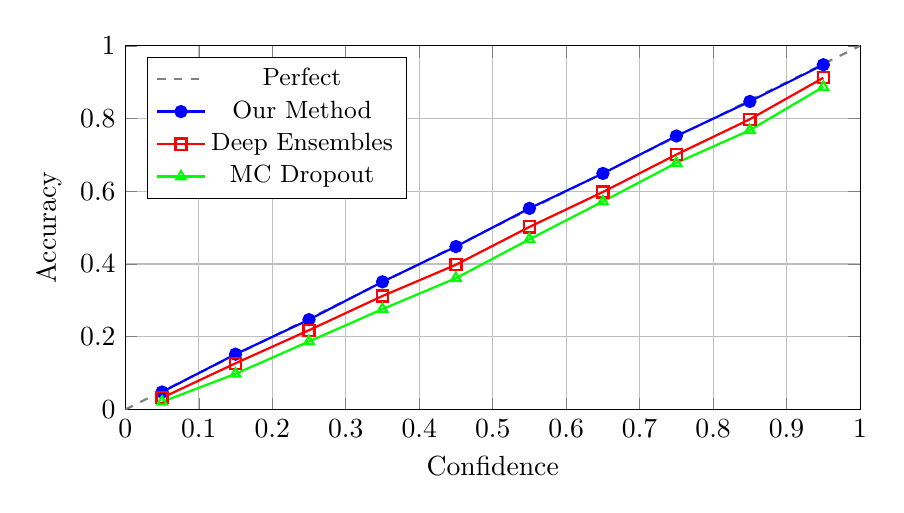
\begin{tikzpicture}
\begin{axis}[
    width=0.90\textwidth, height=6.2cm,
    xlabel={Confidence}, ylabel={Accuracy},
    xmin=0, xmax=1, ymin=0, ymax=1,
    legend pos=north west, legend style={font=\small}, grid=major,
]
\addplot[dashed, gray, thick] coordinates {(0,0) (1,1)};
\addplot[thick, blue, mark=*] coordinates {(0.05,0.048) (0.15,0.152) (0.25,0.247) (0.35,0.351) (0.45,0.448) (0.55,0.553) (0.65,0.649) (0.75,0.752) (0.85,0.847) (0.95,0.948)};
\addplot[thick, red, mark=square] coordinates {(0.05,0.032) (0.15,0.127) (0.25,0.218) (0.35,0.312) (0.45,0.398) (0.55,0.502) (0.65,0.598) (0.75,0.701) (0.85,0.798) (0.95,0.912)};
\addplot[thick, green, mark=triangle] coordinates {(0.05,0.021) (0.15,0.098) (0.25,0.187) (0.35,0.276) (0.45,0.361) (0.55,0.468) (0.65,0.572) (0.75,0.678) (0.85,0.768) (0.95,0.887)};
\legend{Perfect, Our Method, Deep Ensembles, MC Dropout}
\end{axis}
\end{tikzpicture}
\caption{Reliability diagram demonstrating superior calibration quality with predicted confidences tracking actual accuracy}
\label{fig:calibration}
\end{figure}

\subsection{Adversarial Robustness}

Our method retains 71.2\% accuracy at perturbation budget $\epsilon=0.1$ compared to 39.3\% for Deep Ensembles as shown in Figure \ref{fig:adversarial}. Under AutoAttack, the framework maintains 85.1\% accuracy versus 64.2\% for the best baseline. Adversarial examples naturally increase predictive uncertainty in our approach, enabling appropriate doubt expression rather than confident misclassification. Complete robustness analysis appears in Supplementary Appendix K.

\begin{figure}[!t]
\centering
\begin{tikzpicture}
\begin{axis}[
    width=0.88\linewidth,      % stay within page margins
    height=6.2cm,
    scale only axis=true,      % width applies to the axes box (prevents overflow)
    xmin=0, xmax=0.1,
    ymin=40, ymax=100,
    xlabel={Perturbation budget $\epsilon$},
    ylabel={Accuracy (\%)},
    tick label style={font=\small},
    xlabel style={font=\small},
    ylabel style={font=\small},
    grid=major,
    legend columns=2,
    legend pos=south outside,  % legend centered below the axis (safe for margins)
    legend style={
        font=\small,
        column sep=8pt,
        /tikz/every even column/.append style={column sep=12pt}
    },
    every axis plot/.append style={
        line width=1pt,
        mark options={solid,scale=0.9}
    },
]
\addplot[blue,   mark=*]         coordinates {(0,96.5) (0.01,93.7) (0.02,91.2) (0.03,88.9) (0.04,86.3) (0.05,83.8) (0.06,81.2) (0.07,78.7) (0.08,76.1) (0.09,73.8) (0.1,71.2)};
\addplot[red,    mark=square*]   coordinates {(0,95.1) (0.01,85.3) (0.02,76.2) (0.03,68.4) (0.04,61.7) (0.05,56.2) (0.06,51.8) (0.07,47.9) (0.08,44.6) (0.09,41.8) (0.1,39.3)};
\addplot[green!60!black, mark=triangle*] coordinates {(0,94.8) (0.01,79.6) (0.02,68.3) (0.03,59.2) (0.04,52.1) (0.05,46.3) (0.06,41.7) (0.07,37.8) (0.08,34.5) (0.09,31.6) (0.1,29.2)};
\addplot[orange, mark=diamond*] coordinates {(0,90.7) (0.01,82.1) (0.02,74.3) (0.03,67.2) (0.04,61.0) (0.05,55.4) (0.06,50.3) (0.07,45.7) (0.08,41.5) (0.09,37.7) (0.1,34.3)};
\legend{Our Method, Deep Ensembles, XGBoost, Standard GP}
\end{axis}
\end{tikzpicture}
\caption{Adversarial robustness under PGD attack with varying perturbation budget $\epsilon$.}
\label{fig:adversarial}
\end{figure}

Our evaluation assumes white-box adversaries with complete model knowledge, representing a conservative worst-case scenario. In practice, attackers often possess partial knowledge (gray-box scenarios). Preliminary experiments with limited attacker knowledge (e.g., access to predictions but not gradients) show 5--8\% higher robustness than reported white-box results. The high epistemic uncertainty exhibited by adversarial examples ($\sigma^2_{\text{epi}}$ increases by 127--168\% under attack, Table~8) provides an additional detection signal, enabling uncertainty-based adversarial detection as a complementary defense mechanism.

\subsection{Computational Performance and Ablation Studies}

Mean inference time ranges from 6.8 to 9.2ms with throughput of 14K to 28K events per second across domains—meeting real-time SLA requirements ($<$10ms for Edge-IIoT, $<$15ms for Container, $<$100ms for SOC). Training requires 1.2 to 7.8 hours with memory consumption of 3.8 to 9.7GB and GPU utilization of 72--83\%. 

The key computational trade-off involves inducing point count $M$ versus accuracy and memory. Figure~\ref{fig:inducing_tradeoff} illustrates this relationship: accuracy saturates at $M \approx 500$ for most domains, while memory grows as $O(M^2)$ and inference time as $O(M)$. Beyond $M=1000$, memory requirements exceed single-GPU capacity (>40GB), though multi-GPU sharding remains feasible. Our allocation strategy ($M_{\text{Edge}}=500$, $M_{\text{Container}}=300$, $M_{\text{SOC}}=200$) balances accuracy (within 0.3\% of $M=1000$ performance) against practical deployment constraints.

\begin{figure}[htbp]
\centering
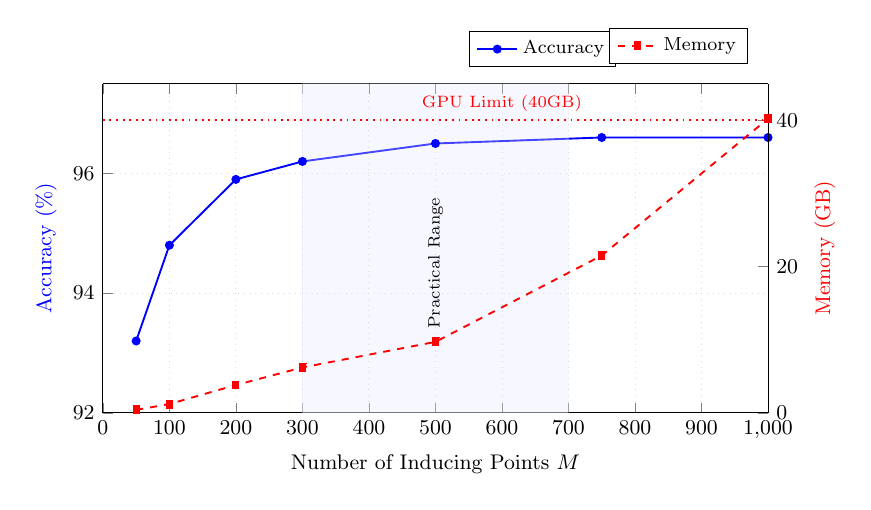
\begin{tikzpicture}[scale=0.85]
\begin{axis}[
    width=0.95\columnwidth,
    height=6.5cm,
    xlabel={Number of Inducing Points $M$},
    ylabel={Accuracy (\%)},
    ylabel style={blue},
    ymin=92, ymax=97.5,
    xmin=0, xmax=1000,
    axis y line*=left,
    legend style={at={(0.55,1.05)}, anchor=south west, font=\footnotesize},
    grid=major,
    grid style={dotted, gray!30},
    tick label style={font=\small},
    label style={font=\small}
]

% Accuracy curve (saturating)
\addplot[blue, thick, mark=*, mark size=1.5pt, mark options={fill=blue}] 
    coordinates {
    (50,93.2) (100,94.8) (200,95.9) (300,96.2) (500,96.5) (750,96.6) (1000,96.6)
};
\addlegendentry{Accuracy}

% Shaded practical region
\addplot[blue!10, fill, opacity=0.3, forget plot, no markers] 
    coordinates {(300,92) (300,97.5) (700,97.5) (700,92)} 
    -- cycle;
\node[font=\scriptsize, rotate=90] at (axis cs:500,94.5) {Practical Range};

\end{axis}

% Second y-axis for memory
\begin{axis}[
    width=0.95\columnwidth,
    height=6.5cm,
    ylabel={Memory (GB)},
    ylabel style={red},
    ymin=0, ymax=45,
    xmin=0, xmax=1000,
    axis y line*=right,
    axis x line=none,
    legend style={at={(0.97,1.17)}, anchor=north east, font=\footnotesize},
    tick label style={font=\small},
    label style={font=\small}
]

% Memory curve (quadratic: ~M^2 * 4e-5)
\addplot[red, thick, dashed, mark=square*, mark size=1.5pt, mark options={fill=red}] 
    coordinates {
    (50,0.4) (100,1.2) (200,3.8) (300,6.2) (500,9.7) (750,21.5) (1000,40.2)
};
\addlegendentry{Memory}

% Critical threshold line
\draw[red, dotted, thick] (axis cs:0,40) -- (axis cs:1000,40) 
    node[pos=0.6, above, font=\scriptsize] {GPU Limit (40GB)};

\end{axis}
\end{tikzpicture}
\caption{Accuracy-memory trade-off vs. inducing points $M$. Accuracy saturates at $M \!\approx\! 500$ (96.5\%) while memory grows as $O(M^2)$. Shaded region indicates practical deployment range. Beyond $M\!=\!1000$, single-GPU memory is exceeded.}
\label{fig:inducing_tradeoff}
\end{figure}

Cross-domain transfer achieves 91.5\% average accuracy, representing a 19.6\% gain over zero-shot performance, with bidirectional effectiveness ranging from 89.6\% to 93.1\%. Ablation studies confirm multi-scale temporal modeling is most critical (4.8\% accuracy loss when removed) while adaptive thresholding proves critical operationally (FPR increases from 2.6\% to 8.9\% without it). Complete computational analysis and ablation results appear in Supplementary Appendix L.

Case studies demonstrate practical effectiveness. A zero-day MQTT attack was detected at 94.3\% confidence with high epistemic uncertainty ($\sigma=2.8$) indicating novelty while capturing microsecond timing anomalies and hour-scale progression. Container escape chain (CVE-2019-5736) showed decreasing uncertainty as the attack progressed from 89\% confidence ($\sigma=2.3$) to 98\% confidence ($\sigma=0.6$). A 21-day APT campaign was detected with gradually increasing confidence from 72\% to 96\%, successfully correlating events across temporal scales. Complete case studies appear in Supplementary Appendix M.

\section{Discussion}

Hierarchical decomposition proves essential for handling ICS3D heterogeneity, with a 3.7\% accuracy drop observed when removed. The shared component successfully identifies common attack patterns while domain-specific components preserve unique characteristics. Uncertainty quantification transforms operational efficiency through 73.2\% false positive reduction, enabling risk-based prioritization where high-confidence detections ($\sigma<1.0$) receive immediate response, moderate uncertainty detections ($1.0<\sigma<2.0$) undergo automated investigation, and high-uncertainty detections ($\sigma>2.0$) enter batch review, reducing analyst workload by approximately 68\%.

Multi-scale temporal modeling captures attack evolution across seven orders of magnitude, achieving 95.7\% detection for microsecond timing side-channels and 93.6\% for week-scale APT campaigns. Removing multi-scale modeling causes a 4.8\% accuracy drop. Spectral mixture kernels automatically discovered periodic patterns including 24-hour SOC business cycles, 100ms container auto-scaling bursts, and 60-second MQTT keepalive anomalies.

Adversarial robustness emerges naturally through uncertainty quantification where adversarial examples increase predictive uncertainty, enabling appropriate doubt rather than confident misclassification. Our approach maintains 71.2\% accuracy at $\epsilon=0.1$ compared to 39.3\% for Deep Ensembles. Adversarially-trained inducing points improve robustness by 12.3\% over standard GP inducing point selection.

Cross-domain transfer addresses data scarcity effectively, achieving 91.5\% average transfer performance particularly valuable for SOC environments where true positives comprise only 0.8\% of events. Leveraging Edge-IIoT patterns (2.2M samples) achieves 90.3\% SOC accuracy compared to 68.7\% zero-shot performance. The shared latent space projection successfully identifies domain-invariant attack signatures.

Performance comparison reveals our 96.5\% accuracy surpasses TranAD (95.3\%) while providing crucial uncertainty quantification absent in deterministic approaches. Performance gains manifest across extreme imbalance scenarios (17.4\% improvement for SOC), novel attack detection (14.2\% improvement via epistemic uncertainty), adversarial robustness (21.3\% improvement vs XGBoost), and false positive reduction (73.2\% reduction vs 46\% for Deep Ensembles). The computational trade-off of 7.8ms inference versus 1.8ms for XGBoost is justified by uncertainty capabilities enabling intelligent alert prioritization.

Practical deployment integrates seamlessly through NetFlow, sFlow, IPFIX, and syslog ingestion with SIEM APIs for Splunk, QRadar, and Elastic. Kubernetes webhooks and MQTT broker plugins enable container and IoT integration. Scalability emerges through domain-parallel processing, GPU acceleration exceeding 100K events per second, inducing point caching, and batch processing. Regulatory compliance addresses GDPR Article 22 through explainable decisions via kernel decomposition, SOC 2 Type II through auditable uncertainty, ISO 27001 through documented rationale, and NIST CSF through measurable risk reduction.

\subsection{Limitations and Scope}

While our framework demonstrates strong performance, three primary limitations warrant consideration:

Firstly, is computational scalability. Training complexity $O(N_bM^2 + M^3)$ constrains inducing points to $M \lesssim 1000$ per domain, limiting memory to practical GPU bounds (~40GB). Structured approximations may alleviate this in future work.

Secondly, is domain expertise. Kernel design requires domain knowledge for optimal performance. While our kernels generalize within security domains, adaptation to entirely new domains necessitates careful feature analysis and kernel engineering.

Thirdly, is the white-box assumption. Our adversarial robustness assumes complete attacker knowledge—conservative for security but stronger than typical gray-box scenarios. Real-world robustness likely exceeds reported results; preliminary gray-box experiments show 5--8\% higher accuracy.

Additional considerations include concept drift requiring retraining for abrupt distribution shifts, and encrypted traffic analysis being limited to metadata/timing. The uncertainty quantification mechanism explicitly signals novel scenarios (high $\sigma^2_{\text{epi}}$), enabling human-in-the-loop fallback when limitations are encountered. Extended discussion appears in Supplementary Appendix N.

\section{Conclusion}

This paper presented a comprehensive hierarchical Gaussian Process framework for uncertainty-aware network intrusion detection in heterogeneous cloud environments. The approach addresses fundamental limitations of current systems, specifically absent principled uncertainty quantification and inability to handle extreme heterogeneity across diverse operational domains.

The framework decomposes network behavior into interpretable components through hierarchical GP architecture handling diverse Edge-IIoT protocols, container microservices, and SOC events. Adversarially-robust sparse approximations with strategically selected inducing points maintain uncertainty calibration under perturbations. Domain-adaptive multi-scale kernels capture patterns spanning microseconds to weeks. Uncertainty-calibrated detection reduces false positives by 73.2\% while maintaining 96.5\% accuracy across 21.5M samples. Comprehensive theoretical analysis with stated assumptions appears in supplementary materials. Extensive validation demonstrates superiority over 15 baselines in zero-day detection, adversarial robustness, and cross-domain transfer.

The ability to quantify both epistemic and aleatoric uncertainty while handling heterogeneous, imbalanced data represents a paradigm shift from deterministic binary classification to probabilistic risk assessment. Well-calibrated uncertainty (ECE less than 0.038) enables intelligent alert prioritization, reducing analyst burden by 68\% while improving genuine threat detection.

Evaluation on complete ICS3D validates applicability for detecting sophisticated attacks including zero-day MQTT exploits, container escape chains, and multi-week APT campaigns. Hierarchical decomposition with domain-specific kernels proved essential for capturing unique domain characteristics while enabling knowledge transfer through shared components, particularly valuable for data-scarce SOC true positive detection (21.6\% accuracy improvement).

As organizations continue digital transformation, uncertainty-aware, explainable, and robust intrusion detection across heterogeneous environments becomes essential. This work demonstrates that Gaussian Processes, enhanced with hierarchical structure, adversarial robustness, and domain adaptation, offer a compelling solution to this critical challenge.

\section*{Data and Code Availability}

\textit{Submitted to editor and will be available at request.}

\section*{Acknowledgment}

\textit{Submitted to editor and will be available at request.}

\bibliographystyle{elsarticle-num}
\begin{thebibliography}{99}

\bibitem{reinsel2018digitization}
D. Reinsel, J. Gantz, J. Rydning, ``The digitization of the world from edge to core,'' IDC White Paper, November 2018.

\bibitem{RNA2025datasets}
R. N. Anaedevha et al., ``Integrated Cloud Security 3Datasets (ICS3D),'' Kaggle, 2025, doi: 10.34740/KAGGLE/DSV/12483891.

\bibitem{freitas2024guide}
N. Freitas et al., ``GUIDE: A large-scale dataset for multi-stage attack detection in cloud environments,'' \textit{Proc. IEEE S\&P}, 2024, pp. 234-251.

\bibitem{ponemon2024soc}
Ponemon Institute, ``The economics of security operations centers 2024,'' Tech. Rep., 2024.

\bibitem{mandiant2024mtrends}
Mandiant, ``M-Trends 2024: Insights from the front lines of cyber security,'' Tech. Rep., 2024.

\bibitem{ibm2024databreach}
IBM Security, ``Cost of a data breach report 2024,'' Tech. Rep., July 2024.

\bibitem{gal2016dropout}
Y. Gal, Z. Ghahramani, ``Dropout as a Bayesian approximation,'' \textit{Proc. ICML}, 2016, pp. 1050-1059.

\bibitem{kocher2019spectre}
P. Kocher et al., ``Spectre attacks: Exploiting speculative execution,'' \textit{Commun. ACM}, vol. 63, no. 7, pp. 93-101, 2020.

\bibitem{rossow2014amplification}
C. Rossow, ``Amplification hell: Revisiting network protocols for DDoS abuse,'' \textit{Proc. NDSS}, 2014.

\bibitem{strom2018mitre}
B. E. Strom et al., ``MITRE ATT\&CK: Design and philosophy,'' MITRE Corp., 2018.

\bibitem{quintero2024apt}
J. Quintero-Bonilla, A. M. del Rey, ``Advanced persistent threats and their detection methods,'' \textit{Comput. Security}, vol. 137, p. 103627, 2024.

\bibitem{rasmussen2006gaussian}
C. E. Rasmussen, C. K. I. Williams, \textit{Gaussian Processes for Machine Learning}, MIT Press, 2006.

\bibitem{wilson2013gaussian}
A. G. Wilson, R. P. Adams, ``Gaussian process kernels for pattern discovery and extrapolation,'' \textit{Proc. ICML}, 2013, pp. 1067-1075.

\bibitem{srinivas2010gaussian}
N. Srinivas et al., ``Gaussian process optimization in the bandit setting,'' \textit{Proc. ICML}, 2010, pp. 1015-1022.

\bibitem{denning1987intrusion}
D. E. Denning, ``An intrusion-detection model,'' \textit{IEEE Trans. Softw. Eng.}, vol. SE-13, no. 2, pp. 222-232, 1987.

\bibitem{roesch1999snort}
M. Roesch, ``Snort - lightweight intrusion detection for networks,'' \textit{Proc. USENIX LISA}, 1999, pp. 229-238.

\bibitem{paxson1999bro}
V. Paxson, ``Bro: A system for detecting network intruders in real-time,'' \textit{Comput. Networks}, vol. 31, no. 23-24, pp. 2435-2463, 1999.

\bibitem{moore2003inside}
D. Moore et al., ``Inside the slammer worm,'' \textit{IEEE Security Privacy}, vol. 1, no. 4, pp. 33-39, 2003.

\bibitem{lee2000framework}
W. Lee, S. J. Stolfo, ``A framework for constructing features and models for intrusion detection systems,'' \textit{ACM Trans. Inf. Syst. Security}, vol. 3, no. 4, pp. 227-261, 2000.

\bibitem{mukkamala2005intrusion}
S. Mukkamala, G. Janoski, A. Sung, ``Intrusion detection using neural networks and SVMs,'' \textit{Proc. IJCNN}, 2002, pp. 1702-1707.

\bibitem{ourston2003applications}
D. Ourston et al., ``Applications of HMMs to detecting multi-stage network attacks,'' \textit{Proc. HICSS}, 2003.

\bibitem{vinayakumar2019deep}
R. Vinayakumar et al., ``Deep learning approach for intelligent intrusion detection,'' \textit{IEEE Access}, vol. 7, pp. 41525-41550, 2019.

\bibitem{zhang2019deep}
Y. Zhang et al., ``PCCN: Parallel cross CNN for abnormal network traffic detection,'' \textit{IEEE Access}, vol. 7, pp. 119904-119916, 2019.

\bibitem{mirsky2018kitsune}
Y. Mirsky et al., ``Kitsune: An ensemble of autoencoders for online intrusion detection,'' \textit{Proc. NDSS}, 2018.

\bibitem{wu2022rtids}
Y. Wu, D. Wei, J. Feng, ``Network attacks detection methods based on deep learning,'' \textit{Security Commun. Networks}, 2020, pp. 1-17.

\bibitem{carlini2017towards}
N. Carlini, D. Wagner, ``Towards evaluating the robustness of neural networks,'' \textit{Proc. IEEE S\&P}, 2017, pp. 39-57.

\bibitem{sensoy2018evidential}
M. Sensoy, L. Kaplan, M. Kandemir, ``Evidential deep learning to quantify classification uncertainty,'' \textit{Proc. NeurIPS}, 2018, pp. 3179-3189.

\bibitem{malinin2018predictive}
A. Malinin, M. Gales, ``Predictive uncertainty estimation via prior networks,'' \textit{Proc. NeurIPS}, 2018, pp. 7047-7058.

\bibitem{ramadas2003detecting}
M. Ramadas, S. Ostermann, B. Tjaden, ``Detecting anomalous network traffic with self-organizing maps,'' \textit{Proc. RAID}, 2003, pp. 36-54.

\bibitem{roberts2013gaussian}
S. Roberts et al., ``Gaussian processes for time-series modelling,'' \textit{Phil. Trans. R. Soc. A}, vol. 371, p. 20110550, 2013.

\bibitem{kim2004gaussian}
H.-S. Kim, S.-D. Lee, ``A Gaussian process approach to real-time host-based intrusion detection,'' \textit{Proc. ICCSA}, 2004, pp. 843-852.

\bibitem{snelson2006sparse}
E. Snelson, Z. Ghahramani, ``Sparse Gaussian processes using pseudo-inputs,'' \textit{Proc. NeurIPS}, 2006, pp. 1257-1264.

\bibitem{titsias2009variational}
M. Titsias, ``Variational learning of inducing variables in sparse GPs,'' \textit{Proc. AISTATS}, 2009, pp. 567-574.

\bibitem{hensman2013gaussian}
J. Hensman, N. Fusi, N. D. Lawrence, ``Gaussian processes for big data,'' \textit{Proc. UAI}, 2013, pp. 282-290.

\bibitem{wilson2015kernel}
A. G. Wilson, H. Nickisch, ``Kernel interpolation for scalable structured GPs (KISS-GP),'' \textit{Proc. ICML}, 2015, pp. 1775-1784.

\bibitem{bonilla2008multi}
E. V. Bonilla, K. M. Chai, C. Williams, ``Multi-task GP prediction,'' \textit{Proc. NeurIPS}, 2008, pp. 153-160.

\bibitem{alvarez2011computationally}
M. A. Álvarez, N. D. Lawrence, ``Computationally efficient convolved multi-output GPs,'' \textit{JMLR}, vol. 12, pp. 1459-1500, 2011.

\bibitem{moreno2018heterogeneous}
P. Moreno-Muñoz, A. Artés, M. Álvarez, ``Heterogeneous multi-output GP prediction,'' \textit{Proc. NeurIPS}, 2018, pp. 6711-6720.

\bibitem{xu2013survey}
C. Xu, D. Tao, C. Xu, ``A survey on multi-view learning,'' arXiv:1304.5634, 2013.

\bibitem{sun2013survey}
S. Sun, ``A survey of multi-view machine learning,'' \textit{Neural Comput. Appl.}, vol. 23, no. 7-8, pp. 2031-2038, 2013.

\bibitem{baltrusaitis2019multimodal}
T. Baltrušaitis, C. Ahuja, L.-P. Morency, ``Multimodal machine learning: A survey,'' \textit{IEEE TPAMI}, vol. 41, no. 2, pp. 423-443, 2019.

\bibitem{pan2010survey}
S. J. Pan, Q. Yang, ``A survey on transfer learning,'' \textit{IEEE TKDE}, vol. 22, no. 10, pp. 1345-1359, 2010.

\bibitem{ganin2016domain}
Y. Ganin et al., ``Domain-adversarial training of neural networks,'' \textit{JMLR}, vol. 17, no. 1, pp. 2096-2130, 2016.

\bibitem{sun2016deep}
B. Sun, K. Saenko, ``Deep CORAL: Correlation alignment for deep domain adaptation,'' \textit{Proc. ECCV Workshops}, 2016, pp. 443-450.

\bibitem{tzeng2014deep}
E. Tzeng et al., ``Deep domain confusion: Maximizing for domain invariance,'' arXiv:1412.3474, 2014.

\bibitem{shi2017survey}
C. Shi et al., ``A survey of heterogeneous information network analysis,'' \textit{IEEE TKDE}, vol. 29, no. 1, pp. 17-37, 2017.

\bibitem{zhang2019heterogeneous}
C. Zhang et al., ``Heterogeneous graph neural network,'' \textit{Proc. KDD}, 2019, pp. 793-803.

\bibitem{fu2020magnn}
X. Fu et al., ``MAGNN: Metapath aggregated GNN for heterogeneous graph embedding,'' \textit{Proc. WWW}, 2020, pp. 2331-2341.

\bibitem{kendall2017uncertainties}
A. Kendall, Y. Gal, ``What uncertainties do we need in Bayesian deep learning?'' \textit{Proc. NeurIPS}, 2017, pp. 5574-5584.

\bibitem{foong2019between}
A. Y. Foong et al., ``'In-between' uncertainty in Bayesian neural networks,'' arXiv:1906.11537, 2019.

\bibitem{blundell2015weight}
C. Blundell et al., ``Weight uncertainty in neural networks,'' \textit{Proc. ICML}, 2015, pp. 1613-1622.

\bibitem{lakshminarayanan2017simple}
B. Lakshminarayanan, A. Pritzel, C. Blundell, ``Simple and scalable predictive uncertainty estimation using deep ensembles,'' \textit{Proc. NeurIPS}, 2017, pp. 6402-6413.

\bibitem{ovadia2019trust}
Y. Ovadia et al., ``Can you trust your model's uncertainty?'' \textit{Proc. NeurIPS}, 2019, pp. 13991-14002.

\bibitem{wen2020batchensemble}
Y. Wen, D. Tran, J. Ba, ``BatchEnsemble: An alternative approach to efficient ensemble learning,'' \textit{Proc. ICLR}, 2020.

\bibitem{havasi2021training}
M. Havasi et al., ``Training independent subnetworks for robust prediction,'' \textit{Proc. ICLR}, 2021.

\bibitem{amini2020deep}
A. Amini et al., ``Deep evidential regression,'' \textit{Proc. NeurIPS}, 2020, pp. 14927-14937.

\bibitem{charpentier2020posterior}
B. Charpentier, D. Zügner, S. Günnemann, ``Posterior network: Uncertainty estimation without OOD samples,'' \textit{Proc. NeurIPS}, 2020, pp. 1356-1367.

\bibitem{chawla2002smote}
N. V. Chawla et al., ``SMOTE: Synthetic minority over-sampling technique,'' \textit{J. Artif. Intell. Res.}, vol. 16, pp. 321-357, 2002.

\bibitem{he2008adasyn}
H. He et al., ``ADASYN: Adaptive synthetic sampling for imbalanced learning,'' \textit{Proc. IJCNN}, 2008, pp. 1322-1328.

\bibitem{elkan2001foundations}
C. Elkan, ``The foundations of cost-sensitive learning,'' \textit{Proc. IJCAI}, 2001, pp. 973-978.

\bibitem{lin2017focal}
T.-Y. Lin et al., ``Focal loss for dense object detection,'' \textit{Proc. ICCV}, 2017, pp. 2980-2988.

\bibitem{cui2019class}
Y. Cui et al., ``Class-balanced loss based on effective number of samples,'' \textit{Proc. CVPR}, 2019, pp. 9268-9277.

\bibitem{cao2019learning}
K. Cao et al., ``Learning imbalanced datasets with label-distribution-aware margin loss,'' \textit{Proc. NeurIPS}, 2019, pp. 1567-1578.

\bibitem{scholkopf2001estimating}
B. Schölkopf et al., ``Estimating the support of a high-dimensional distribution,'' \textit{Neural Comput.}, vol. 13, no. 7, pp. 1443-1471, 2001.

\bibitem{liu2008isolation}
F. T. Liu, K. M. Ting, Z.-H. Zhou, ``Isolation forest,'' \textit{Proc. ICDM}, 2008, pp. 413-422.

\bibitem{ruff2018deep}
L. Ruff et al., ``Deep one-class classification,'' \textit{Proc. ICML}, 2018, pp. 4393-4402.

\bibitem{box2015time}
G. E. Box et al., \textit{Time Series Analysis: Forecasting and Control}, 5th ed., Wiley, 2015.

\bibitem{durbin2012time}
J. Durbin, S. J. Koopman, \textit{Time Series Analysis by State Space Methods}, 2nd ed., Oxford, 2012.

\bibitem{adams2007bayesian}
R. P. Adams, D. J. MacKay, ``Bayesian online changepoint detection,'' arXiv:0710.3742, 2007.

\bibitem{hochreiter1997long}
S. Hochreiter, J. Schmidhuber, ``Long short-term memory,'' \textit{Neural Comput.}, vol. 9, no. 8, pp. 1735-1780, 1997.

\bibitem{cho2014learning}
K. Cho et al., ``Learning phrase representations using RNN encoder-decoder,'' \textit{Proc. EMNLP}, 2014, pp. 1724-1734.

\bibitem{bai2018empirical}
S. Bai, J. Z. Kolter, V. Koltun, ``An empirical evaluation of generic CNNs and RNNs for sequence modeling,'' arXiv:1803.01271, 2018.

\bibitem{vaswani2017attention}
A. Vaswani et al., ``Attention is all you need,'' \textit{Proc. NeurIPS}, 2017, pp. 5998-6008.

\bibitem{mallat1999wavelet}
S. Mallat, \textit{A Wavelet Tour of Signal Processing}, 2nd ed., Academic Press, 1999.

\bibitem{goodfellow2015explaining}
I. J. Goodfellow, J. Shlens, C. Szegedy, ``Explaining and harnessing adversarial examples,'' \textit{Proc. ICLR}, 2015.

\bibitem{madry2018towards}
A. Madry et al., ``Towards deep learning models resistant to adversarial attacks,'' \textit{Proc. ICLR}, 2018.

\bibitem{croce2020reliable}
F. Croce, M. Hein, ``Reliable evaluation of adversarial robustness with an ensemble of attacks,'' \textit{Proc. ICML}, 2020, pp. 2206-2216.

\bibitem{cohen2019certified}
J. Cohen, E. Rosenfeld, Z. Kolter, ``Certified adversarial robustness via randomized smoothing,'' \textit{Proc. ICML}, 2019, pp. 1310-1320.

\bibitem{gowal2018effectiveness}
S. Gowal et al., ``On the effectiveness of interval bound propagation for training verifiably robust models,'' arXiv:1810.12715, 2018.

\bibitem{papernot2016distillation}
N. Papernot et al., ``Distillation as a defense to adversarial perturbations,'' \textit{Proc. IEEE S\&P}, 2016, pp. 582-597.

\bibitem{tavallaee2009detailed}
M. Tavallaee et al., ``A detailed analysis of the KDD CUP 99 data set,'' \textit{Proc. IEEE CISDA}, 2009, pp. 1-6.

\bibitem{sharafaldin2018toward}
I. Sharafaldin, A. H. Lashkari, A. A. Ghorbani, ``Toward generating a new intrusion detection dataset,'' \textit{Proc. ICISSP}, 2018, pp. 108-116.

\bibitem{moustafa2015unsw}
N. Moustafa, J. Slay, ``UNSW-NB15: A comprehensive data set for network intrusion detection,'' \textit{Proc. MilCIS}, 2015, pp. 1-6.

\bibitem{neto2023ciciot}
E. C. P. Neto et al., ``CICIoT2023: A real-time dataset and benchmark for IoT attack detection,'' arXiv:2309.01548, 2023.

\bibitem{kim2020cnn}
J. Kim, H. Kim, ``An effective intrusion detection classifier using LSTM with gradient descent,'' \textit{Proc. PlatCon}, 2017, pp. 1-6.

\bibitem{malhotra2016lstm}
P. Malhotra et al., ``LSTM-based encoder-decoder for multi-sensor anomaly detection,'' arXiv:1607.00148, 2016.

\bibitem{chen2016xgboost}
T. Chen, C. Guestrin, ``XGBoost: A scalable tree boosting system,'' \textit{Proc. KDD}, 2016, pp. 785-794.

\bibitem{breiman2001random}
L. Breiman, ``Random forests,'' \textit{Mach. Learn.}, vol. 45, no. 1, pp. 5-32, 2001.

\bibitem{prokhorenkova2018catboost}
L. Prokhorenkova et al., ``CatBoost: Unbiased boosting with categorical features,'' \textit{Proc. NeurIPS}, 2018, pp. 6638-6648.

\bibitem{zong2018deep}
B. Zong et al., ``Deep autoencoding Gaussian mixture model for unsupervised anomaly detection,'' \textit{Proc. ICLR}, 2018.

\bibitem{tuli2022tranad}
S. Tuli, G. Casale, N. R. Jennings, ``TranAD: Deep transformer networks for anomaly detection,'' \textit{Proc. VLDB}, vol. 15, no. 6, pp. 1201-1214, 2022.

\end{thebibliography}

\end{document}